% =====================================================================
\chapter{Cointégration}
\label{ch:4}
% =====================================================================

\section{Objectifs et organisation du chapitre}

\paragraph{Objectifs.} Le chapitre~1 a donné l'intuition de la cointégration ; ce chapitre en donne la théorie et les outils. À la fin, vous saurez : (1) définir l'ordre d'intégration et la cointégration ; (2) appliquer la méthode d'Engle-Granger avec les bonnes valeurs critiques ; (3) expliquer la superconvergence du ratio de couverture et ses limites ; (4) écrire un modèle à correction d'erreur et en déduire qui \og corrige\fg{} l'écart et à quelle vitesse ; (5) comprendre la procédure de Johansen pour plusieurs actifs ; (6) reconnaître une cointégration partielle ; (7) appliquer le tout aux paires réelles du cours.

\paragraph{Code.} \texttt{code/ch04/ch04\_cointegration.py}, expériences E1 à E6.

% =====================================================================
\section{Ordre d'intégration et définition}
% =====================================================================

\begin{definition}[Ordre d'intégration]
Une série $x_t$ est \emph{intégrée d'ordre $d$}, notée $x_t\sim I(d)$, s'il faut la différencier $d$ fois pour obtenir une série stationnaire (sans tendance déterministe non modélisée). Une série stationnaire est $I(0)$ ; une marche aléatoire est $I(1)$, puisque $\Delta x_t = \varepsilon_t$ est $I(0)$.
\end{definition}

\begin{definition}[Cointégration, \citet{englegranger1987}]
Les composantes d'un vecteur $x_t = (x_{1t},\dots,x_{kt})^\top$, toutes $I(1)$, sont \emph{cointégrées} s'il existe un vecteur non nul $\beta\in\R^k$ tel que $\beta^\top x_t$ soit $I(0)$. Le vecteur $\beta$ est un \emph{vecteur de cointégration} ; le nombre $r$ de vecteurs linéairement indépendants qui ont cette propriété est le \emph{rang de cointégration}, avec $0\le r < k$.
\end{definition}

Pour deux actifs, $r$ vaut 0 (pas de relation) ou 1 (une relation), et le vecteur est défini à un facteur près ; on le \emph{normalise} en fixant le coefficient d'un actif à 1 : $\beta = (1, -\beta_2)$, d'où l'écart $S_t = x_{1t} - \beta_2x_{2t}$.

\begin{intuition}
Pensez à $k$ bateaux sur une mer agitée. La marée (une tendance stochastique commune) les soulève tous. S'il y a $k$ bateaux mais seulement $k-r$ marées indépendantes, il existe $r$ combinaisons de leurs hauteurs dans lesquelles les marées s'annulent : ce sont les écarts stationnaires. Deux bateaux sur la même marée : une combinaison. Deux bateaux dans deux ports différents : aucune.
\end{intuition}

% =====================================================================
\section{La méthode d'Engle-Granger}
% =====================================================================

\subsection{Les deux étapes}

\begin{enumerate}
\item \textbf{Estimer} la relation de long terme par MCO : $x_{1t} = a + b\,x_{2t} + e_t$ (chapitre~2).
\item \textbf{Tester} la stationnarité des résidus $\hat e_t$ par un test de Dickey-Fuller augmenté (chapitre~3), \emph{avec des valeurs critiques spécifiques}.
\end{enumerate}

\subsection{Pourquoi des valeurs critiques spécifiques}

À la première étape, les MCO choisissent $b$ pour que les résidus soient \emph{les plus petits possible}. Même si $x_1$ et $x_2$ ne sont pas cointégrés, ces résidus ont donc l'air \og plus stationnaires\fg{} qu'une marche aléatoire quelconque : la régression a déjà fait une partie du travail du test. Il faut donc des seuils plus exigeants. Avec deux variables et une constante, les valeurs asymptotiques de \citet{englegranger1987}, affinées par MacKinnon, sont $-3{,}90$ (1\,\%), $-3{,}34$ (5\,\%) et $-3{,}04$ (10\,\%) ; avec trois variables, $-4{,}29$ ; $-3{,}74$ ; $-3{,}45$.

\begin{codebox}[ — E1, valeurs critiques d'Engle-Granger]
\textbf{Protocole :} 10\,000 paires de marches aléatoires indépendantes de 500 points ; régression puis Dickey-Fuller sur les résidus. \textbf{Résultats :} quantiles simulés $-3{,}91$ ; $-3{,}36$ ; $-3{,}07$, conformes aux valeurs tabulées. Avec le seuil de Dickey-Fuller ($-2{,}86$), on déclarerait cointégrées $14{,}9\,\%$ des paires indépendantes, trois fois le taux nominal ; avec le seuil d'Engle-Granger, $5{,}3\,\%$.
\end{codebox}

\begin{figure}[h]
\centering
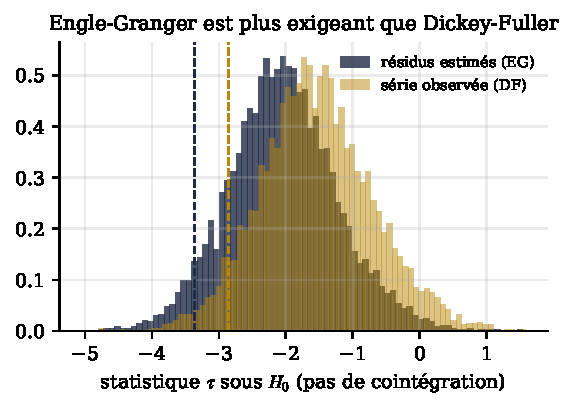
\includegraphics[width=0.62\textwidth]{ch04/eg_distribution.pdf}
\caption{Sous l'hypothèse d'absence de cointégration, la statistique calculée sur des résidus estimés (Engle-Granger) est décalée vers la gauche par rapport à celle d'une série observée (Dickey-Fuller).}
\label{c4:fig:eg}
\end{figure}

\subsection{La superconvergence du ratio}

Quand la paire est réellement cointégrée, l'estimateur MCO de $b$ converge vers la vraie valeur à la vitesse $1/n$, et non $1/\sqrt n$ comme dans une régression ordinaire : on parle de \emph{superconvergence}. L'intuition : le régresseur $x_2$ erre de plus en plus loin (sa variance empirique croît comme $n$), ce qui rend toute erreur sur $b$ de plus en plus coûteuse en somme des carrés.

\begin{codebox}[ — E2, superconvergence]
\textbf{Protocole :} vrai $b = 1{,}5$, écart AR(1) avec $\varphi = 0{,}9$, 500 répétitions. \textbf{Résultats :} écart-type de $\hat b$ : $0{,}111$ ($n = 250$), $0{,}030$ ($n = 1\,000$), $0{,}0081$ ($n = 4\,000$) ; il est divisé par environ 4 quand $n$ est multiplié par 4 (vitesse $1/n$). Pour une régression entre variables stationnaires : $0{,}067$ ; $0{,}030$ ; $0{,}016$, divisé par 2 seulement (vitesse $1/\sqrt n$).
\end{codebox}

\begin{pitfall}
La superconvergence est un résultat asymptotique qui suppose que la tendance commune domine le bruit de l'écart. Sur deux ans de données, avec un écart volatil, $\hat b$ peut rester loin de la vérité (voir E3 ci-dessous, où $\hat b = 0{,}88$ pour une vraie valeur de 1). Elle ne protège en rien contre une relation qui change au cours du temps.
\end{pitfall}

% =====================================================================
\section{Le modèle à correction d'erreur}
% =====================================================================

\subsection{Le théorème de représentation de Granger}

\begin{theorem}[Représentation de Granger, énoncé simplifié]
Deux séries $I(1)$ sont cointégrées, d'écart $S_t = x_{1t} - \beta x_{2t}$, si et seulement si elles admettent une représentation à correction d'erreur
\begin{align*}
\Delta x_{1t} &= \mu_1 + \alpha_1 S_{t-1} + \text{(retards de } \Delta x_1, \Delta x_2) + \varepsilon_{1t},\\
\Delta x_{2t} &= \mu_2 + \alpha_2 S_{t-1} + \text{(retards de } \Delta x_1, \Delta x_2) + \varepsilon_{2t},
\end{align*}
avec $(\alpha_1,\alpha_2)\ne(0,0)$.
\end{theorem}

Les coefficients $\alpha_1$, $\alpha_2$ sont les \emph{vitesses d'ajustement}. Si l'écart est positif ($x_1$ trop haut par rapport à $x_2$), il faut que $x_1$ baisse ($\alpha_1<0$) ou que $x_2$ monte ($\alpha_2>0$), ou les deux.

\begin{intuition}
Dans l'image de \citet{murray1994}, si la promeneuse appelle son chien et que le chien revient, c'est le chien qui \og corrige l'erreur\fg{} ; si la promeneuse va chercher son chien, c'est elle ; souvent, les deux font la moitié du chemin. Le modèle à correction d'erreur mesure qui fait quoi.
\end{intuition}

\subsection{Vitesse de retour de l'écart}

\begin{proposition}\label{c4:prop:ecm}
Sans retards, l'écart suit $\Delta S_t = (\mu_1 - \beta\mu_2) + (\alpha_1 - \beta\alpha_2)\,S_{t-1} + (\varepsilon_{1t} - \beta\varepsilon_{2t})$. C'est un AR(1) de coefficient $\varphi_S = 1 + \alpha_1 - \beta\alpha_2$.
\end{proposition}
\begin{proof}
$\Delta S_t = \Delta x_{1t} - \beta\Delta x_{2t}$ ; on remplace chaque variation par son équation et on regroupe les termes en $S_{t-1}$. On reconnaît l'écriture \og retour à la moyenne\fg{} de l'AR(1), équation~\eqref{c1:eq:ecm} du chapitre~1, avec $\varphi_S - 1 = \alpha_1 - \beta\alpha_2$.
\end{proof}

\begin{codebox}[ — E3, correction d'erreur]
\textbf{Protocole :} système simulé ($n = 2\,000$) avec $\beta = 1$, $\alpha_1 = -0{,}10$, $\alpha_2 = +0{,}05$ ; donc $\varphi_S = 1 - 0{,}10 - 0{,}05 = 0{,}85$ et une demi-vie de $4{,}27$ jours. \textbf{Résultats :} $\hat\beta = 0{,}879$ ; $\hat\alpha_1 = -0{,}127$ ($t = -13{,}3$) ; $\hat\alpha_2 = 0{,}055$ ($t = 6{,}0$) ; $\hat\varphi_S = 0{,}825$, demi-vie $3{,}6$ jours. Les deux jambes participent à la correction, avec les bons signes. Le biais sur $\beta$ vient de ce que, dans ce système, la tendance commune est faible par rapport au bruit de l'écart.
\end{codebox}

\paragraph{Lecture pour le trading.} Si seule une jambe corrige ($\alpha_2 \approx 0$), l'autre est le \og meneur\fg{} : c'est elle qui porte l'information, et c'est sur la jambe suiveuse que le retour se produit. Pour un \emph{pairs trade}, cela influence le choix de la jambe à exécuter en premier et le risque d'exécution (chapitre~15). Dans le cas \texttt{atjte}, le CFD sur MT5 sert de prix de référence : on suppose implicitement que c'est le prix sur la plateforme crypto qui s'ajuste.

% =====================================================================
\section{Plusieurs actifs : la procédure de Johansen}
% =====================================================================

\subsection{Le VECM}

Avec $k$ actifs, on écrit un modèle vectoriel à correction d'erreur (VECM) :
\[
\Delta x_t = \mu + \Pi\,x_{t-1} + \sum_{i=1}^{p-1}\Gamma_i\,\Delta x_{t-i} + \varepsilon_t, \qquad \Pi = \alpha\beta^\top,
\]
où $\alpha$ et $\beta$ sont des matrices $k\times r$. Les colonnes de $\beta$ sont les vecteurs de cointégration, celles de $\alpha$ les vitesses d'ajustement. Le rang de $\Pi$ est le nombre de relations de cointégration : rang 0, pas de relation (le modèle se réduit à un VAR en différences) ; rang $k$, toutes les séries sont stationnaires ; entre les deux, $r$ relations.

\subsection{L'idée de Johansen}

\citet{johansen1991} estime le VECM par maximum de vraisemblance. Après avoir retiré l'effet des retards $\Delta x_{t-i}$ par régression, il calcule les \emph{corrélations canoniques} entre les variations $\Delta x_t$ et les niveaux $x_{t-1}$ : ce sont les combinaisons des niveaux qui prédisent le mieux les variations. Les carrés de ces corrélations sont des valeurs propres $\hat\lambda_1 \ge \dots \ge \hat\lambda_k$ ; un $\hat\lambda_i$ nettement positif signale une combinaison de niveaux qui \og rappelle\fg{} les prix, donc une relation de cointégration. Deux statistiques testent le rang :
\[
\text{trace}(r) = -T\sum_{i=r+1}^{k}\ln(1-\hat\lambda_i), \qquad \text{valeur propre max}(r) = -T\ln(1-\hat\lambda_{r+1}),
\]
qui testent $H_0$ : rang $\le r$. On teste successivement $r = 0, 1, \dots$ et on s'arrête au premier non-rejet.

\begin{codebox}[ — E4, Johansen sur trois actifs]
\textbf{Protocole :} $x_1$ et $x_2$ partagent une tendance commune ($x_2 = 0{,}5\times$ tendance $+$ AR(1)), $x_3$ suit sa propre tendance ; une seule relation, $x_2 - 0{,}5x_1$. \textbf{Résultats :} statistique de trace $48{,}1$ ; $6{,}1$ ; $2{,}1$ pour $r = 0, 1, 2$, contre des seuils à 5\,\% de $29{,}8$ ; $15{,}5$ ; $3{,}8$ : on rejette $r = 0$, pas $r = 1$ : rang 1, correct. Vecteur estimé normalisé sur $x_2$ : $(-0{,}535\,;\,1\,;\,-0{,}042)$, proche de $(-0{,}5\,;\,1\,;\,0)$.
\end{codebox}

\paragraph{Engle-Granger ou Johansen ?} Engle-Granger est simple et transparent mais dépend du choix de la variable normalisée et ne trouve qu'une relation ; Johansen traite les actifs symétriquement et estime le nombre de relations, mais il est sensible à la spécification (retards, termes déterministes) et ses propriétés sur petits échantillons sont moins bonnes. En \emph{pairs trading}, on utilise souvent Engle-Granger pour la sélection et Johansen pour les paniers de trois actifs et plus.

% =====================================================================
\section{La cointégration partielle}
% =====================================================================

Les paires réelles ne sont presque jamais parfaitement cointégrées : leur relation dérive lentement (changement de modèle économique, de structure de coûts). \citet{clegg2018} modélisent l'écart comme la somme de deux composantes cachées,
\[
S_t = M_t + R_t, \qquad M_t = \rho M_{t-1} + \varepsilon^M_t,\quad R_t = R_{t-1} + \varepsilon^R_t,
\]
une partie qui revient à la moyenne ($|\rho|<1$, écart-type d'innovation $\sigma_M$) et une partie marche aléatoire (écart-type $\sigma_R$). Comme $R$ est une marche aléatoire, $S$ n'est pas stationnaire : un test de cointégration classique conclut à l'absence de relation. Pourtant, une partie des variations de l'écart est prévisible.

\begin{proposition}\label{c4:prop:r2mr}
La part de la variance des variations de l'écart due à la composante de retour à la moyenne vaut
\[
R^2_{MR} = \frac{\Var(\Delta M_t)}{\Var(\Delta S_t)} = \frac{2\sigma_M^2}{2\sigma_M^2 + (1+\rho)\sigma_R^2}.
\]
\end{proposition}
\begin{proof}
D'après la démonstration de la proposition~\ref{c3:prop:vr} avec $q=1$, $\Var(\Delta M_t) = 2\gamma_M(0)(1-\rho) = 2\frac{\sigma_M^2}{1-\rho^2}(1-\rho) = \frac{2\sigma_M^2}{1+\rho}$. Par ailleurs $\Var(\Delta R_t) = \sigma_R^2$, et les deux composantes sont indépendantes, donc $\Var(\Delta S_t) = \frac{2\sigma_M^2}{1+\rho} + \sigma_R^2$. On fait le rapport et on multiplie numérateur et dénominateur par $1+\rho$.
\end{proof}

\begin{codebox}[ — E5, ADF face à la cointégration partielle]
\textbf{Protocole :} $\rho = 0{,}9$, $\sigma_M = 1$, $n = 1\,000$, 300 répétitions. \textbf{Résultats :} pour $\sigma_R = 0$ ; $0{,}1$ ; $0{,}2$ ; $0{,}4$ ; $0{,}8$, on a $R^2_{MR} = 1$ ; $0{,}991$ ; $0{,}963$ ; $0{,}868$ ; $0{,}622$ et le test ADF conclut à la stationnarité dans $100$ ; $98{,}7$ ; $86{,}7$ ; $53{,}3$ ; $17{,}7\,\%$ des cas. Une marche aléatoire qui ne représente que 13\,\% de la variance des variations suffit à rendre le test aveugle une fois sur deux.
\end{codebox}

L'estimation de $(\rho,\sigma_M,\sigma_R)$ se fait par filtre de Kalman, puisque $M$ et $R$ sont des états cachés : ce sera l'objet du chapitre~8.

% =====================================================================
\section{Études de cas réelles}
% =====================================================================

\begin{table}[h]
\centering\small
\caption{Tests de cointégration sur les log-prix (E6).}
\label{c4:tab:real}
\begin{tabular}{lccc}
\toprule
Test & Statistique & $p$-valeur & Seuil 5\,\% \\
\midrule
Engle-Granger, GLD sur GLDM, constante & $-0{,}53$ & 0,962 & $-3{,}35$ \\
Engle-Granger, GLD sur GLDM, tendance & $-22{,}17$ & $<0{,}001$ & $-3{,}80$ \\
Johansen GLD/GLDM avec tendance, trace $r=0$ & $214{,}4$ & — & $18{,}4$ \\
Engle-Granger, KO sur PEP & $-1{,}18$ & 0,864 & $-3{,}35$ \\
Engle-Granger, PEP sur KO & $-3{,}17$ & 0,075 & $-3{,}35$ \\
Johansen KO/PEP, trace $r=0$ & $9{,}99$ & — & $15{,}49$ \\
\bottomrule
\end{tabular}
\end{table}

\paragraph{GLD/GLDM.} Les conclusions du chapitre~3 se confirment : cointégration écrasante dès qu'on autorise la tendance due à l'écart de frais, aucune sinon. Johansen, avec un terme déterministe adapté, trouve aussi une relation.

\paragraph{KO/PEP.} Selon le sens de la régression, la $p$-valeur d'Engle-Granger passe de $0{,}864$ à $0{,}075$ : l'asymétrie du chapitre~2 se répercute sur le test. Johansen, symétrique, ne trouve pas de relation. Conclusion honnête : rien sur cette période ne justifie de traiter KO et PEP comme une paire cointégrée ; un trader qui aurait choisi le sens \og PEP sur KO\fg{} parce qu'il donne la meilleure $p$-valeur aurait fait, sans le savoir, deux tests et retenu le meilleur.

% =====================================================================
\section{Ce que la théorie apporte, et ses limites}
% =====================================================================

\paragraph{Apports.} La cointégration donne une justification statistique précise au \emph{pairs trading} : un écart stationnaire entre deux prix non stationnaires. Le modèle à correction d'erreur relie l'écart à la dynamique de chaque jambe et donne sa vitesse de retour ; Johansen étend le cadre aux paniers.

\paragraph{Limites.} (1) Les tests héritent du manque de puissance du chapitre~3 : sur deux ans, une relation réelle mais lente passe inaperçue. (2) La cointégration est une propriété \og pour toujours\fg{} ; les marchés offrent au mieux des relations temporaires, d'où l'intérêt de la cointégration partielle et des modèles à paramètres variables (chapitre~8). (3) Le choix du sens, des termes déterministes et des retards multiplie les tests implicites. (4) Une relation statistique sans raison économique (même secteur, même sous-jacent, contrainte contractuelle) a peu de chances de survivre hors échantillon.

% =====================================================================
\section{Fiche à recopier au tableau blanc}
% =====================================================================

\begin{whiteboard}
\begin{itemize}[leftmargin=1.2em]
\item \textbf{$I(d)$ :} différencier $d$ fois pour être stationnaire. Prix $\sim I(1)$.
\item \textbf{Cointégration :} $x\sim I(1)$, $\beta^\top x\sim I(0)$ ; rang $r$ = nombre de relations indépendantes.
\item \textbf{Engle-Granger :} MCO en niveaux, puis ADF sur résidus ; seuils 5\,\% : $-3{,}34$ (2 var.), $-3{,}74$ (3 var.).
\item \textbf{Superconvergence :} $\hat b - b = O(1/n)$ si la paire est cointégrée.
\item \textbf{Correction d'erreur :} $\Delta x_{1t} = \alpha_1S_{t-1}+\dots$, $\Delta x_{2t} = \alpha_2S_{t-1}+\dots$ ; $\varphi_S = 1+\alpha_1-\beta\alpha_2$.
\item \textbf{VECM :} $\Delta x_t = \Pi x_{t-1} + \sum\Gamma_i\Delta x_{t-i} + \varepsilon_t$, $\Pi = \alpha\beta^\top$, rang $r$.
\item \textbf{Johansen :} trace $= -T\sum_{i>r}\ln(1-\hat\lambda_i)$ ; tester $r = 0, 1, \dots$
\item \textbf{Cointégration partielle :} $S = M + R$ ; $R^2_{MR} = 2\sigma_M^2/(2\sigma_M^2 + (1+\rho)\sigma_R^2)$.
\end{itemize}
\end{whiteboard}

% =====================================================================
\section{Exercices}
% =====================================================================

\begin{exercise}
Montrez que si $x_t\sim I(1)$ et $y_t = 2x_t + u_t$ avec $u_t$ stationnaire, alors $y_t\sim I(1)$ et $(1,-2)$ est un vecteur de cointégration. Le vecteur $(2,-4)$ en est-il un aussi ?
\end{exercise}

\begin{exercise}
Dans un modèle à correction d'erreur avec $\beta = 1$, $\alpha_1 = -0{,}02$ et $\alpha_2 = 0$, calculez la demi-vie de l'écart. Quelle jambe faut-il surveiller pour anticiper la fermeture de l'écart ?
\end{exercise}

\begin{exercise}
Que se passe-t-il dans la proposition~\ref{c4:prop:ecm} si $\alpha_1 = \beta\alpha_2$ ? Interprétez.
\end{exercise}

\begin{exercise}
Avec $\rho = 0{,}8$ et $\sigma_M = 1$, quelle valeur de $\sigma_R$ donne $R^2_{MR} = 0{,}5$ ?
\end{exercise}

\begin{exercise}[à coder]
Écrivez votre propre fonction \texttt{engle\_granger(y, x)} qui renvoie $\hat b$, la statistique ADF des résidus et une décision au seuil $-3{,}34$, et comparez-la à \texttt{statsmodels.tsa.stattools.coint} sur E1 et E6.
\end{exercise}

\begin{exercise}[à coder]
Estimez le VECM complet de GLD/GLDM avec \texttt{statsmodels.tsa.vector\_ar.vecm.VECM}. Quelle jambe corrige l'écart ? Est-ce cohérent avec la liquidité relative des deux fonds ?
\end{exercise}

% =====================================================================
\section{Pour aller plus loin}
% =====================================================================

\begin{toread}
\begin{itemize}[leftmargin=1.2em]
\item \citet{englegranger1987} : définition, théorème de représentation et méthode en deux étapes.
\item \citet{johansen1991} : la procédure du maximum de vraisemblance ; \citet{hamilton1994}, chapitres~19 (\og Cointegration\fg) et~20 (\og Full-Information Maximum Likelihood Analysis of Cointegrated Systems\fg) pour une présentation pas à pas.
\item \citet{vidyamurthy2004} : la cointégration appliquée au \emph{pairs trading}, avec la notion de tendance commune.
\item \citet{clegg2018} : la cointégration partielle et son estimation.
\item \citet{chan2013}, chapitre~2 : Engle-Granger et Johansen sur des paires d'ETF, avec code.
\end{itemize}
\end{toread}

\section{Scripts du chapitre}
\noindent\texttt{code/ch04/ch04\_cointegration.py} : E1 (figure~\ref{c4:fig:eg}), E2 (superconvergence), E3 (correction d'erreur), E4 (Johansen), E5 (cointégration partielle), E6 (tableau~\ref{c4:tab:real}).
